\documentclass[11pt, a4paper]{article}
\input{preamble.tex}
\switchlang{ru}
\begin{document}

\title{1984 "--- Dave Brown Dual Joystick}
\date{}
\maketitle
\selectlanguage{russian}

Джойстик Dave Brown Dual (рис. \ref{fig:DaveBrownJoystickPic}) --- это сдвоенный двухосевой джойстик, копирующий внешний вид и конструктивные особенности пультов от радиоуправляемых моделей самолётов 80-х годов. Однако, вместо использования  радиоинтерфейса, джойстик является проводным, созданным специально для программы-авиасимулятора Dave Brown RC Flight Simulator, написанной энтузиастом авиамоделирования Джоном Каллендом \cite{Kallend1, Kallend2}. Этот авиасимулятор был доступен на компьютерах Apple II и Commodore 64 в первой половине 1980-х годов, и еще дольше --- на IBM-совместимых компьютерах (встречаются коробочные версии Dave Brown R/C Simulator 1995 года, укомплектованные данным джойстиком). В рамках симуляции джойстик позволяет контролировать параметры полёта, включая крен, тангаж, скорость и высоту, аналогично тому, как это реализовано в радиоуправляемых моделях. Согласно документации, джойстик имел собственное имя, <<Transmitter>> (от англ. <<передатчик>>) \cite{Joystick1}.

\begin{figure}[h]
   \centering
    
\includegraphics[scale=0.7]{1984_dave_brown_dual_joystick/pic_30.jpg}
    \caption{Джойстик Dave Brown Dual}
    \label{fig:DaveBrownJoystickPic}
\end{figure}

Как уже упоминалось, корпус устройства копирует вид и компоновку пультов управления авиамоделями: он выполнен из листового металла, в виде габаритного прямоугольного блока с двумя независимыми стиками. Как видно на рис. \ref{fig:DaveBrownJoystickTopAndBottom}, нижняя сторона корпуса --- абсолютно плоская, лишена каких-либо элементов, в том числе ножек. На верхней стороне можно видеть две рукоятки, каждая со своей парой триммеров, предназначенных для механической регулировки центрального положения по обеим осям, и две красные кнопки тумблерного типа с фиксацией. Еще одна кнопка находится на дальней от пользователя стороне корпуса, и там же присутствуют два кабеля, подключаемые к компьютеру (один кабель соответствует левому стику, другой --- правому).

\begin{figure}[h]
    \centering
    
\includegraphics[scale=0.4]{1984_dave_brown_dual_joystick/top_15.jpg}
    
\includegraphics[scale=0.4]{1984_dave_brown_dual_joystick/bottom_15.jpg}
    \caption{Джойстик Dave Brown Dual joystick, вид сверху и снизу}
    \label{fig:DaveBrownJoystickTopAndBottom}
\end{figure}

Размер корпуса и эргономику можно оценить по рисункам \ref{fig:DaveBrownJoystickSize} и \ref{fig:DaveBrownJoystickHand}.

Узел джойстика, включая весь электромеханический блок, является стандартным компонентом: их можно найти на некоторых компактных аналоговых джойстиках других компаний того времени, включая самый первый джойстик для Apple II, разработанный Джефом Раскином, а затем выпускавшийся под брендом A2D Company. Cтики довольно удобно использовать, держа их пальцами, в то время как ладонь опирается на корпус (рис. \ref{fig:DaveBrownJoystickHand}), чего нельзя сказать о миниатюрных кнопках.

\begin{figure}[h]
    \centering
    
\includegraphics[scale=0.42]{1984_dave_brown_dual_joystick/size_15.jpg}
    \caption{Джойстик Dave Brown Dual на размерном коврике с шагом сетки 1~см}
    \label{fig:DaveBrownJoystickSize}
\end{figure}

К счастью для пользователя, кнопки не предполагают такого интенсивного использования, как в большинстве компьютерных игр. В рамках симуляции пользователю предоставляется возможность контролировать параметры полета, включая крен, тангаж, скорость и высоту. Согласно документации, игра воспроизводит основные физические характеристики полета моделей самолетов и позволяет выполнять базовые маневры, такие как петли и перевороты, обеспечивая формирование первичной мышечной памяти для управления реальными моделями \cite{Joystick2}. Устройство копирует режим управления, наиболее распространенный в радиоуправляемых моделях самолетов своего времени \cite{Joystick1}. Управление тягой осуществляется движением левого стика вперед и назад, управление рулем направления (рыскание) --- движением левого стика влево и вправо, управление рулем высоты (тангаж) --- движением правого стика вперед и назад (для подъема руля высоты нужно потянуть его назад), а управление элеронами (крен) --- движением правого стика влево и вправо. Левая кнопка в нажатом положении в два раза уменьшает чувствительность по оси для руля высоты, а правая оказывает аналогичное воздействие на управление элеронами. Назначение третьей кнопки инструкция не раскрывает.

\begin{figure}[h]
    \centering
    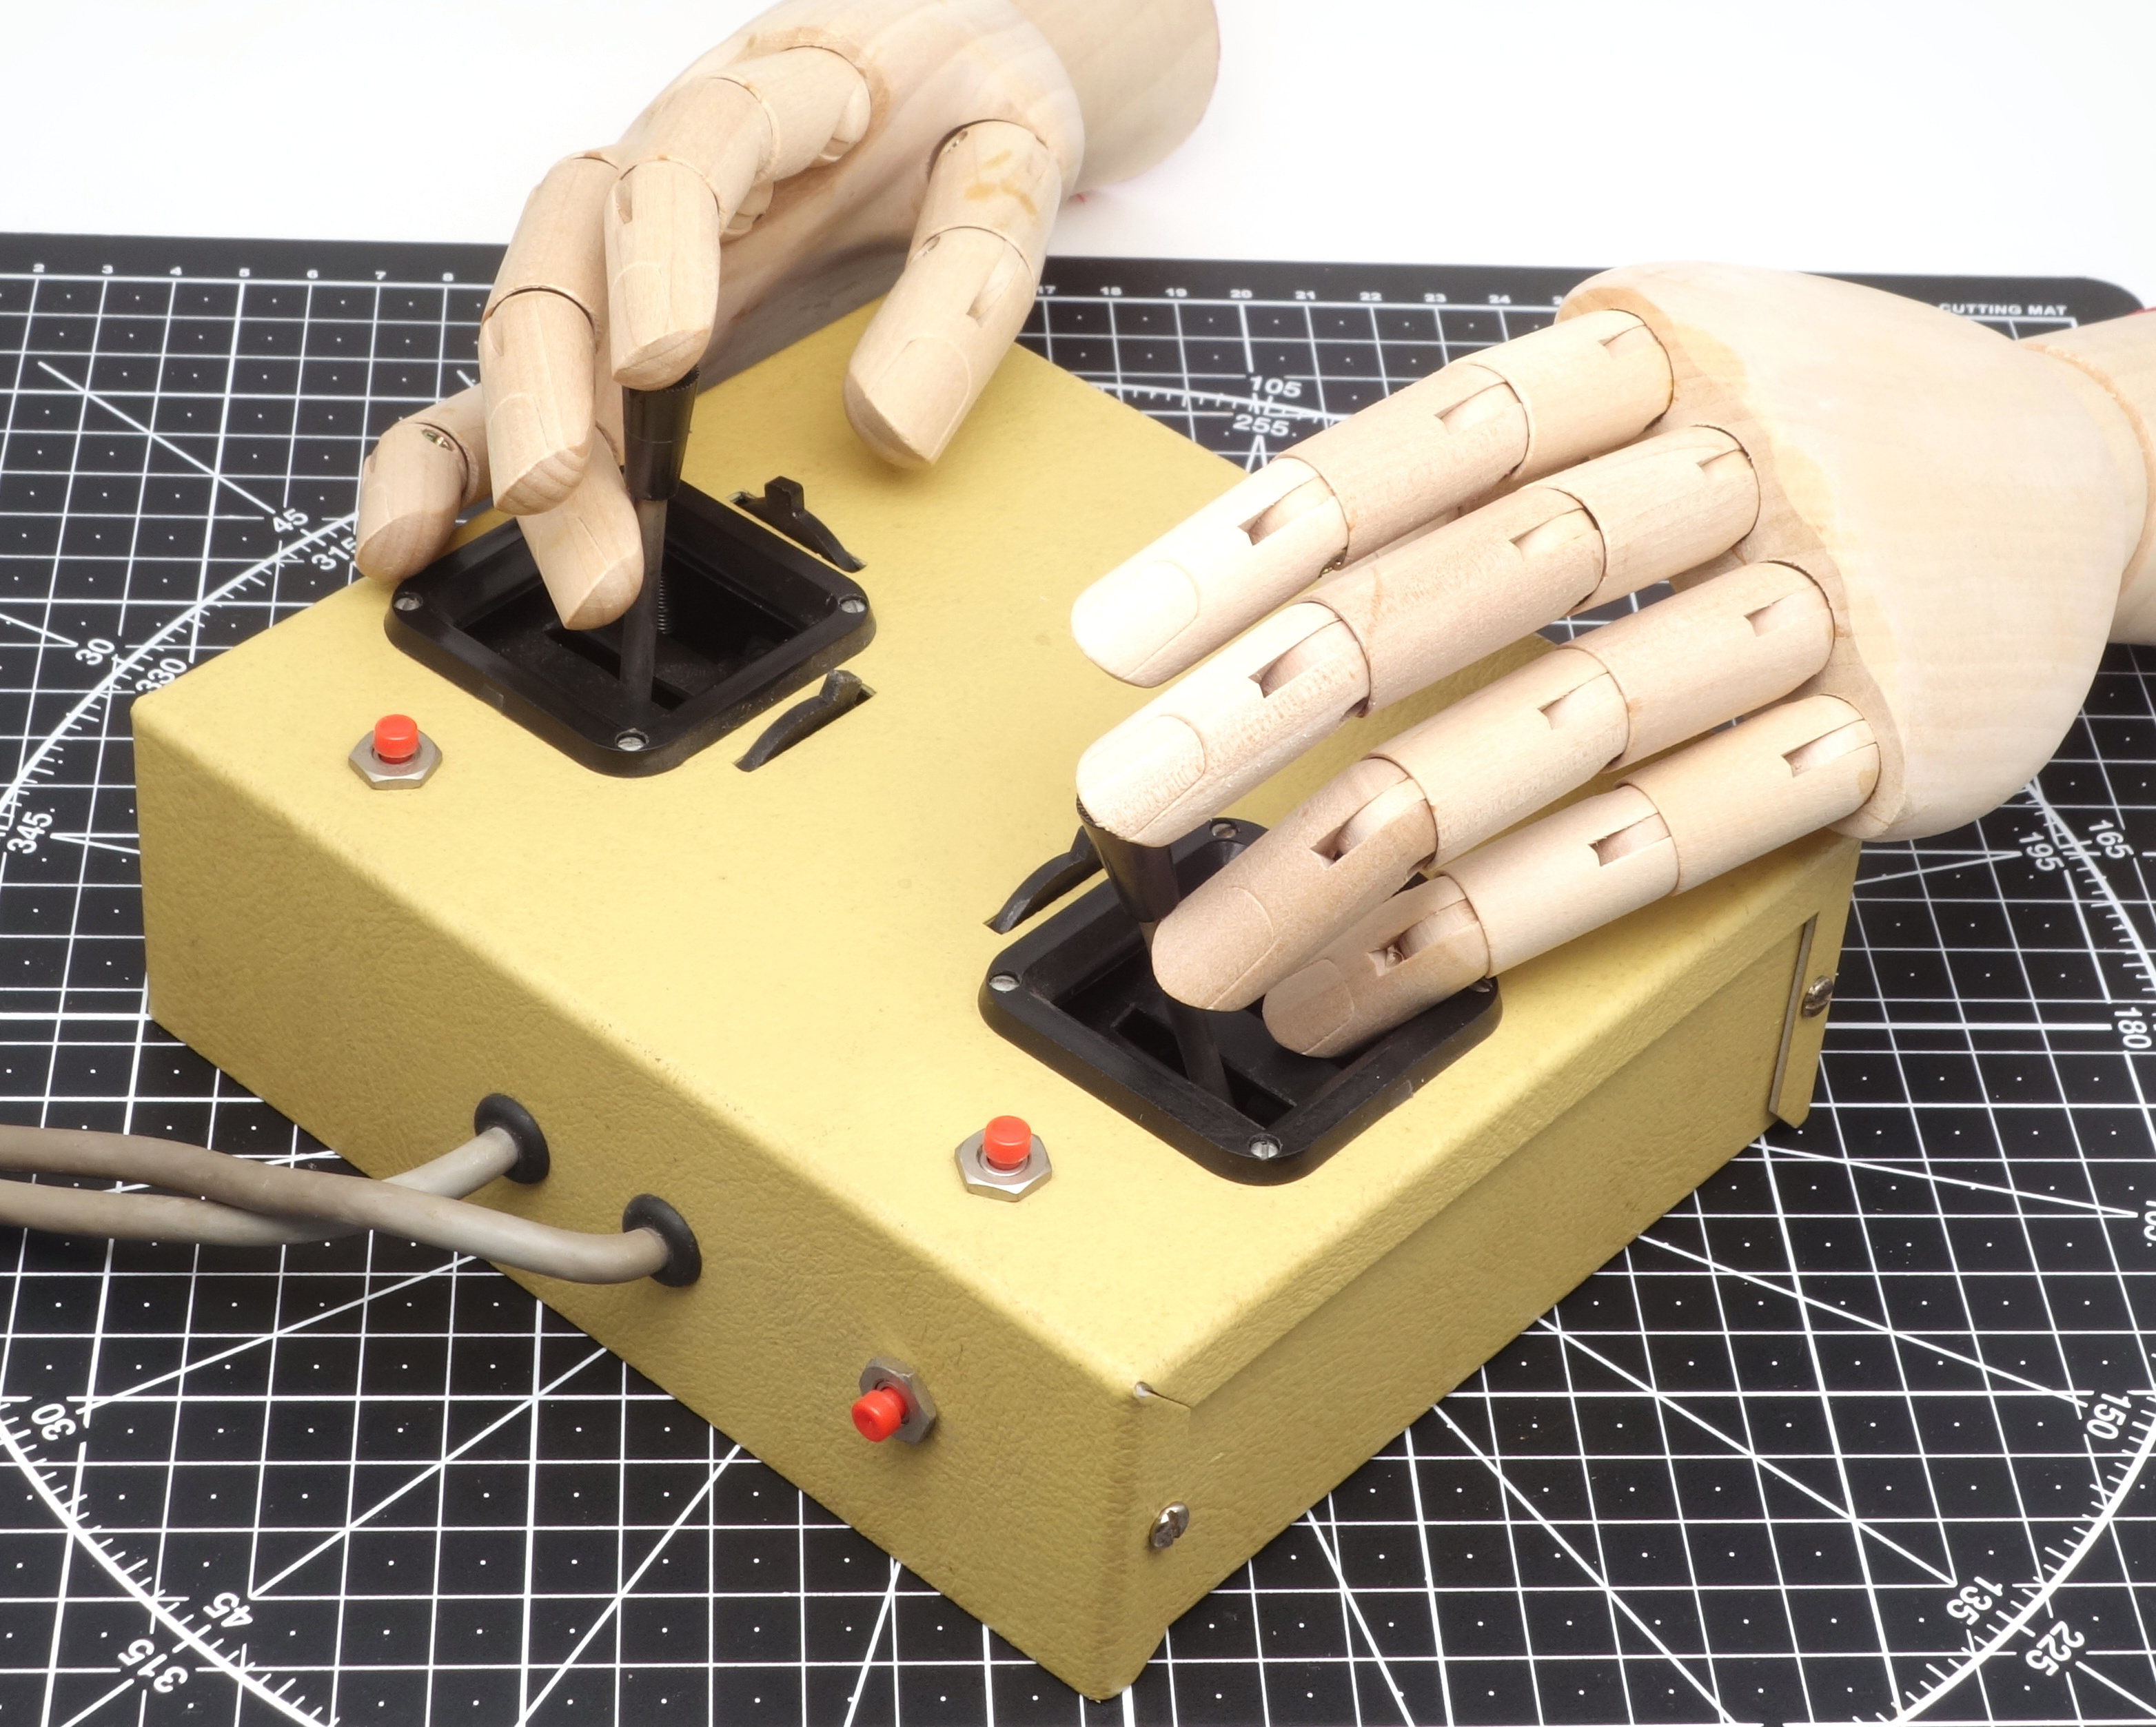
\includegraphics[scale=0.42]{1984_dave_brown_dual_joystick/hand_15.jpg}
    \caption{Джойстик Dave Brown Dual с моделью руки человека}
    \label{fig:DaveBrownJoystickHand}
\end{figure}

Симулятор полета R/C Flight Simulator был разработан для моделирования управления радиоуправляемыми самолетами на экранах 8-битных домашних компьютеров, таких как Apple II и Commodore 64 \cite{Joystick2}.

Как объясняется в руководстве по использованию джойстика \cite{Joystick1} <<пользователю предоставляется реалистичное анимированное изображение модели во время ее «полета», как если бы оно было снято телекамерой, расположенной на земле у ног пилота>>. Далее в том же руководстве поясняется, что <<программа очень сложна, она решает дифференциальные уравнения полета, а затем генерирует 3D-графику в реальном времени>>, однако <<для обеспечения разумной скорости работы программы на микрокомпьютере потребовались некоторые упрощения>>. Действительно, вычислительные возможности 8-битных домашних компьютеров наложили свои ограничения: первое впечатление об особенностях ее графики и уровне детализации можно получить от копии экрана, приведенной на рисунке \ref{fig:game}, а более полно ознакомиться с ней позволяет, например, доступная онлайн версия игры \cite{simulator}. Программное обеспечение представляет интерес еще с той стороны, что его автор Джон Калленд --- вероятно один из старейших энтузиастов авиамоделирования. Во всяком случае, блог, который он вел на ресурсе \url{https://rcgroups.com} после ухода на пенсию с должности профессора кафедры материаловедения Иллинойского технологического института, был активен по июнь 2025 года, а подпись под ником автора скромно сообщала <<Flying R/C since 1964>> \cite{Kallend1}. 

\begin{figure}[h]
    \centering
    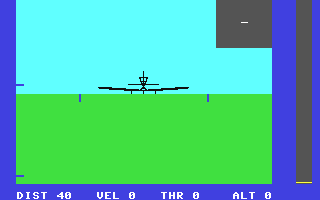
\includegraphics[scale=1]{1984_dave_brown_dual_joystick/screen.png}
    \caption{Копия экрана R/C Flight Simulator} \label{fig:game}
\end{figure}

Внутреннее устройство Dave Brown Dual Joystick показано на рис. \ref{fig:DaveBrownJoystickInside}.  Стики размещены на металлических карданных подвесах (gimbals), обеспечивающих плавное управление по двум осям. Каждый стик соединён с потенциометром, преобразующим отклонение рукоятки в изменение сопротивления. Аналоговый порт Apple II и Commodore 64 \cite{Joystick1} измерял время зарядки RC-цепи, что давало программному обеспечению возможность определить абсолютное положение стика.

\begin{figure}[h]
    \centering
    
\includegraphics[width=\textwidth]{1984_dave_brown_dual_joystick/inside_30.jpg}
    \caption{Джойстик Dave Brown Dual в разобранном виде}
    \label{fig:DaveBrownJoystickInside}
\end{figure}


\begin{thebibliography}{9}
\bibitem {Kallend1} kallend's blog. Do It Yourself Afterburner and other stuff -- RC Groups \url{https://www.rcgroups.com/forums/member.php?u=42040}
\bibitem {Kallend2} Kallend J. The Whistler. Builds great... flights quckly... and is different \url{https://www.rcgroups.com/forums/showatt.php?attachmentid=8106951}
\bibitem {Joystick1} Radio Controlled Flight Simulator By John Kallend For Commodore 64. \url{https://raw.githubusercontent.com/fiowro/mouses/main/source/OCR/dave_brown_simulator_joystick.pdf}
\bibitem {Joystick2} Painful Fun Vintage 1980's Dave Brown RC Flight Simulator | HobbyView \url{https://www.youtube.com/watch?v=zqE4cHVLAhk}
\bibitem {simulator} Play RFC64 -- Radio controlled flight sumulator. CommodoreGames.Net \url{https://www.commodoregames.net/Commodore64/RCFS-64-Radio-Controlled-Flight-Simulator-28134.html}
\end{thebibliography}
\end{document}
